% Source for fig_4_4_3_st_lot.pdf (ST-01). Build: pdflatex fig_4_4_3_st_lot.tex
\documentclass[tikz,border=3pt]{standalone}
\usepackage[T1]{fontenc}\usepackage{lmodern}
\usetikzlibrary{arrows.meta,calc,shapes.geometric}
\newcommand{\diagramfont}{\scriptsize\linespread{1}\selectfont}
\tikzset{
  diagram/.style={x=1mm,y=1mm,font=\diagramfont,>={Stealth[length=1.7mm,width=1.3mm]},line width=0.4pt},
  st/.style={draw,rounded corners=2.5mm,fill=white,minimum width=34mm,minimum height=10mm,align=center,font=\footnotesize\bfseries},
  tl/.style={fill=white,inner sep=0.6mm,align=center,font=\diagramfont},
  ad initial/.style={circle,fill=black,minimum size=3mm,inner sep=0},
  ad final/.style={circle,draw,double,double distance=0.6mm,fill=black,minimum size=2.4mm,inner sep=0}}

\begin{document}
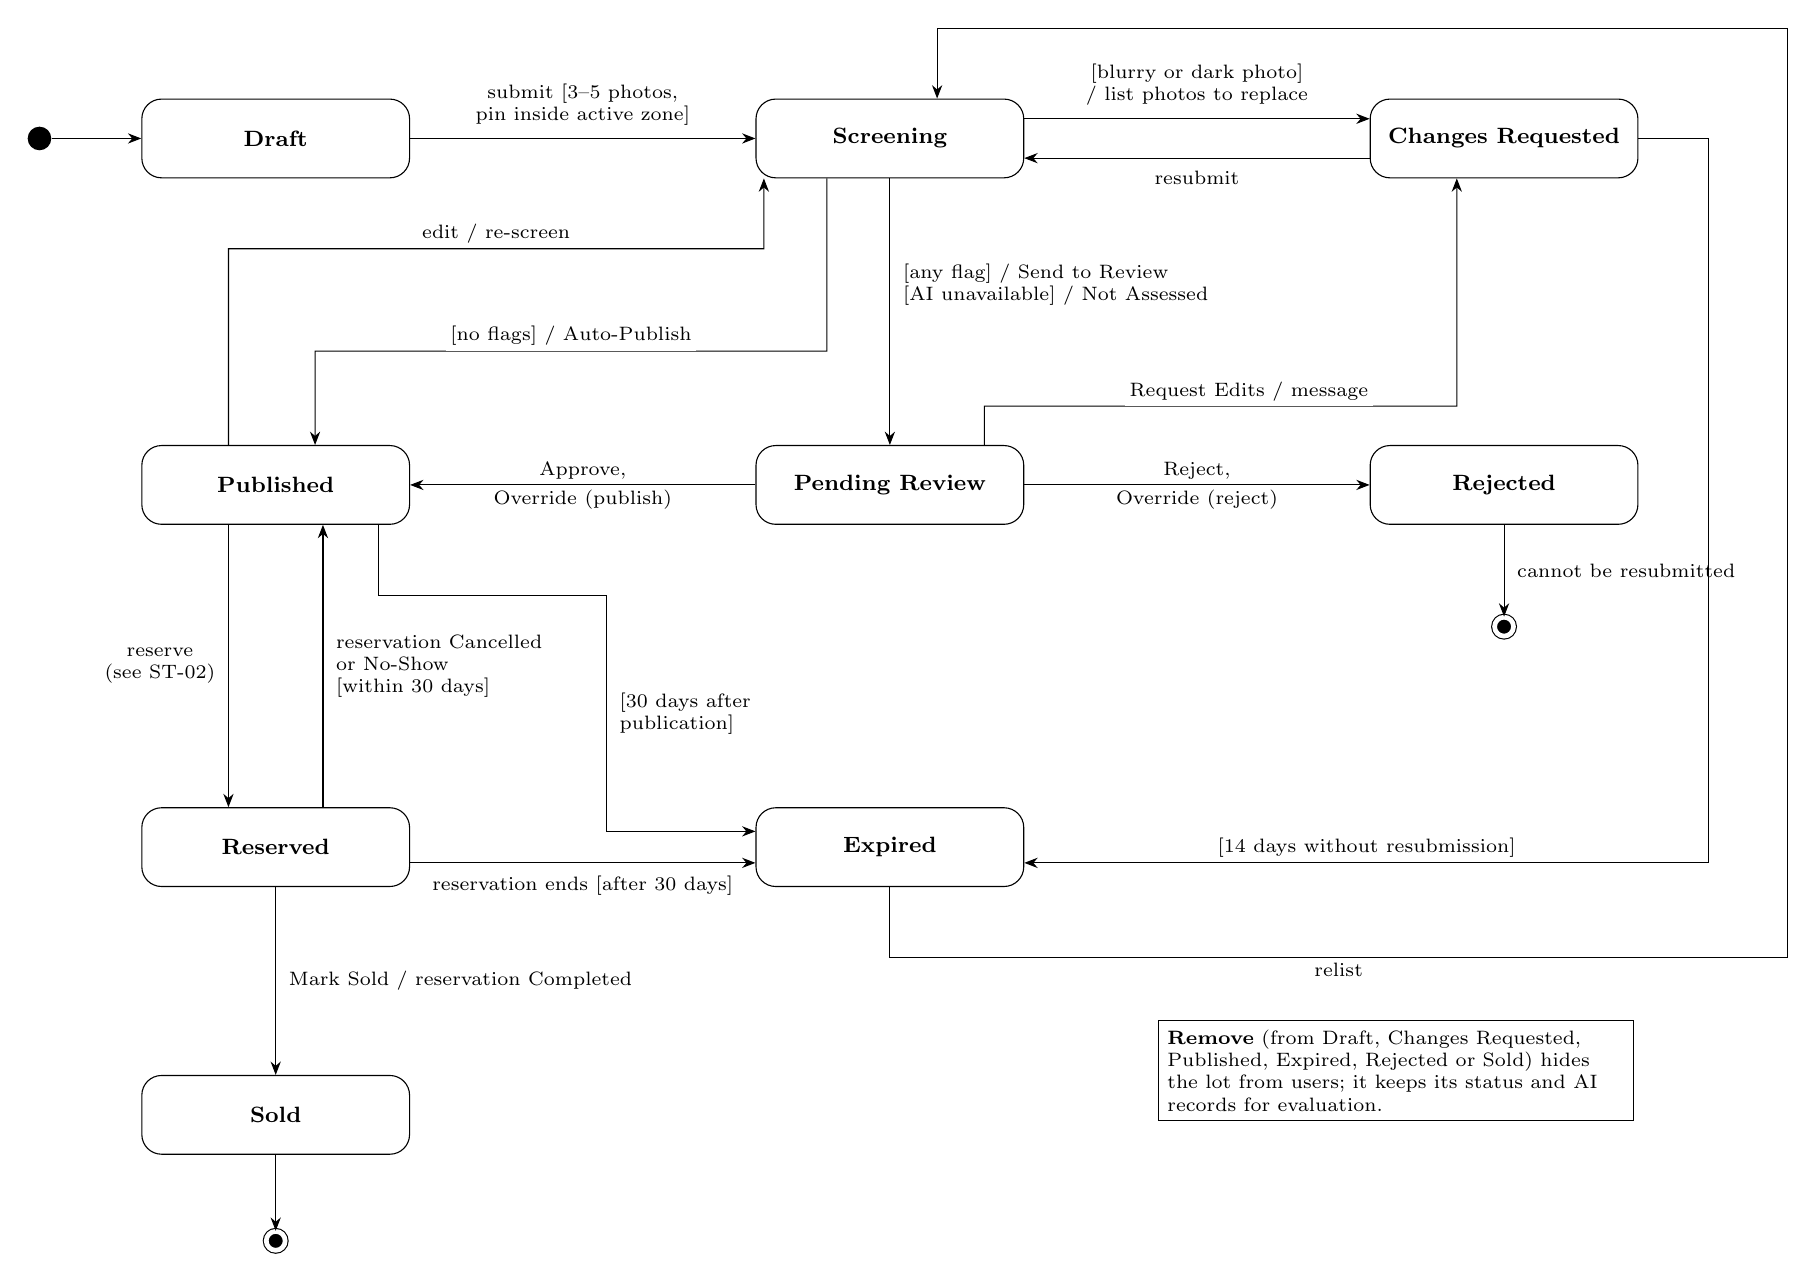
\begin{tikzpicture}[diagram]
  \node[st] (draft) at (0,0) {Draft};
  \node[st] (scr) at (78,0) {Screening};
  \node[st] (cr) at (156,0) {Changes Requested};
  \node[st] (pub) at (0,-44) {Published};
  \node[st] (pr) at (78,-44) {Pending Review};
  \node[st] (rej) at (156,-44) {Rejected};
  \node[st] (res) at (0,-90) {Reserved};
  \node[st] (exp) at (78,-90) {Expired};
  \node[st] (sold) at (0,-124) {Sold};
  \node[ad initial] (i) at (-30,0) {};
  \node[ad final] (fs) at (0,-140) {};
  \node[ad final] (fr) at (156,-62) {};
  % entry and screening
  \draw[->] (i) -- (draft);
  \draw[->] (draft) -- node[tl,above=1mm]{submit [3--5 photos,\\pin inside active zone]} (scr);
  \draw[->] ([yshift=2.5mm]scr.east) -- node[tl,above=1mm]{[blurry or dark photo]\\/ list photos to replace} ([yshift=2.5mm]cr.west);
  \draw[->] ([yshift=-2.5mm]cr.west) -- node[tl,below=1mm]{resubmit} ([yshift=-2.5mm]scr.east);
  \draw[->] (scr.south) -- node[tl,right=1mm,align=left,pos=.4]{[any flag] / Send to Review\\{}[AI unavailable] / Not Assessed} (pr.north);
  \draw[->] ([xshift=-8mm]scr.south) |- (5,-27) node[tl,pos=.75,above]{[no flags] / Auto-Publish} -- ([xshift=5mm]pub.north);
  \draw[->] ([xshift=-6mm]pub.north) |- node[tl,pos=.75,above]{edit / re-screen} (62,-14) -- ([xshift=-16mm]scr.south);
  % review outcomes
  \draw[->] (pr) -- node[tl,above]{Approve,}node[tl,below]{Override (publish)} (pub);
  \draw[->] (pr) -- node[tl,above]{Reject,}node[tl,below]{Override (reject)} (rej);
  \draw[->] ([xshift=12mm]pr.north) |- node[tl,pos=.78,above]{Request Edits / message} (150,-34) -- ([xshift=-6mm]cr.south);
  \draw[->] (rej) -- node[tl,right=1mm]{cannot be resubmitted} (fr);
  \draw[->] (cr.east) -- (182,0) |- node[tl,pos=.75,above]{[14 days without resubmission]} ([yshift=-2mm]exp.east);
  % sale
  \draw[->] ([xshift=-6mm]pub.south) -- node[tl,left=1mm]{reserve\\(see ST-02)} ([xshift=-6mm]res.north);
  \draw[->] ([xshift=6mm]res.north) -- node[tl,right=1mm,align=left]{reservation Cancelled\\or No-Show\\{}[within 30 days]} ([xshift=6mm]pub.south);
  \draw[->] ([xshift=13mm]pub.south) |- (42,-58) |- node[tl,pos=.25,right=1mm,align=left]{[30 days after\\publication]} ([yshift=2mm]exp.west);
  \draw[->] ([yshift=-2mm]res.east) -- node[tl,below=1mm]{reservation ends [after 30 days]} ([yshift=-2mm]exp.west);
  \draw[->] (res) -- node[tl,right=1mm]{Mark Sold / reservation Completed} (sold);
  \draw[->] (sold) -- (fs);
  % relist loop around the diagram
  \draw[->] (exp.south) -- (78,-104) -| node[tl,pos=.25,below]{relist} (192,14) -| ([xshift=6mm]scr.north);
  % remove note
  \node[draw,fill=white,align=left,text width=58mm,anchor=north west] at (112,-112)
    {\textbf{Remove} (from Draft, Changes Requested, Published, Expired, Rejected or Sold) hides the lot from users; it keeps its status and AI records for evaluation.};
\end{tikzpicture}
\end{document}
